\documentclass{article}
\usepackage[utf8]{inputenc}
%Setting page size and margins
\usepackage[a4paper, total={7in, 11in}]{geometry}
\usepackage{multicol}
%Setting stuff to use Russian
\usepackage[T2A]{fontenc}
\usepackage[russian]{babel}
%Pictures
\usepackage{graphicx}
\graphicspath{ {./images/} }

\pagenumbering{gobble}

\title{lab5}
\author{Некруз Назирджанов}
\date{December 2021}

\begin{document}

\begin{minipage}[b]{0.33333\textwidth}
\raggedright
{\large 30}
\end{minipage}%
\begin{minipage}[b]{0.33333\textwidth}
\centering
\textbf{КВАНТ} $\cdot$ \textsf{1999 \slash \textnumero4}
\end{minipage}%

\begin{multicols}{3}
откуда и следует неравенство \\
\[\sum_{i=1}^{n} a_i \sum_{i=1}^{n} c_i \geq (\sum_{i=1}^{n} b_i)^2.\] \par
\textbf{Задача 5.} \textsl{Решите неравенство}
\[\sqrt{|1 - 2x|} \geq 1 + ax.\] \par
\textbf{Решение.}  Очень хотелось бы посмотреть на школьника,
который сумеет записать верное решение этой задачи,
не используя ее геометрической интерпретации. Насколько
трудно это сделать, видно хотя бы из ответа. Чтобы он не
был совсем уж неудобочитаемым, положим для краткости записи\\
\[x_1 = \frac{1 - a - \sqrt{1 - 2a - a^2}}{a^2},\]
\[x_2 = \frac{1 - a + \sqrt{1 - 2a - a^2}}{a^2},\]
\[x_3 = -\frac{2a + 2}{a^2}.\]

Ответ:\\
$x \in [0;+\infty)$ при $a \leq -2;$ \\
$x \in [0;x_3]\bigcup[x_1;+\infty)$ при $2 < a < 0;$ \\
$x \in [x_3;0]\bigcup[x_1;+\infty)$ при $-1\leq a<0;$ \\
$x \in (-\infty;0]\bigcup[1;+\infty)$ при $a=0;$ \\
$x \in (-\infty;0]\bigcup[x_1;x_2]$ при $0 < a \leq \sqrt{2} - 1;$ \\
$x \in (-\infty;0]$ при $a > \sqrt{2} - 1;$ \\
решение понятно из серии графиков, изображенной на рисунке 1. \par
\textbf{Задача 6.} \textsl{Сколько различных каркасов
треугольных пирамид можно со-ставить из зеленых стержней
длиной по 33 см каждый и красных стержней длиной по 20 см?} \par
\textbf{Решение.}  Давайте вначале решим более
простую задачу. Предположим, что зеленые и красные
стержни имеют одинаковую длину. Составим таблицу,
в которой в верхней строке указано
%This is VERY BAD and no one should ever do it like that but i did so deal with it
\begin{minipage}{\linewidth}
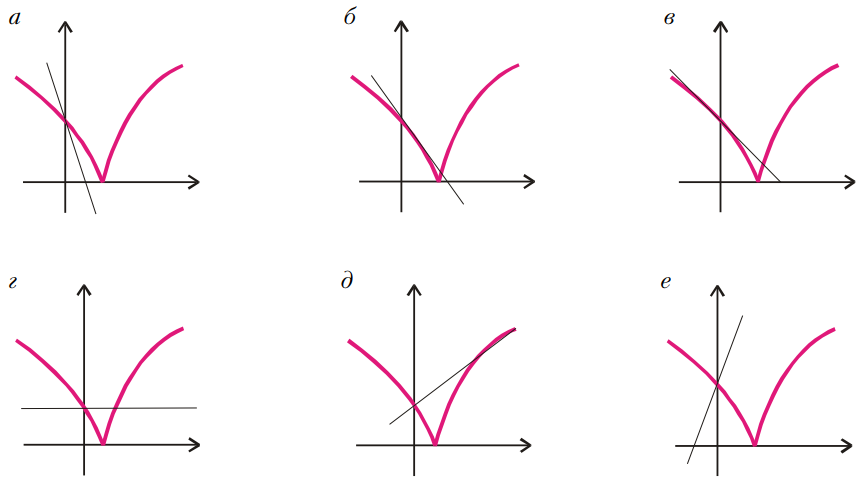
\includegraphics[height=6.4cm]{images/picture1.png} \\
\textsl{Рис. 1} \\
\end{minipage}
число зеленых стержней, а в нижней –
число различно окрашенных пирамид с
таким числом зеленых стержней:
\begin{center}
\begin{tabular}{|c|c|c|c|c|c|c|} 
\hline
0 & 1 & 2 & 3 & 4 & 5 & 6 \\ 
\hline
1 & 1 & 2 & 4 & 2 & 1 & 1 \\
\hline
\end{tabular}
\end{center}
Не кажется ли вам странным число «4» в средней клетке этой таблицы?
Действительно, три зеленых стержня могут: а) выходить из одной вершины;
б) образовывать треугольник; в) образовывать незамкнутую
пространственную ломаную. Однако оказывается, что в случае
в) имеются две различимые конфигурации, правая и левая (рис.2)! \par
Задача в ее исходной постановке отличается от только что разобранной \\ \\
%This is actually not bad at all, feel free to screenshot
\begin{minipage}{\linewidth}
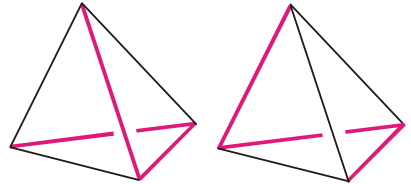
\includegraphics[width=\linewidth]{images/picture2.png} \\
\textsl{Рис. 2} \\
\end{minipage}
тем, что в ней необходимо исследовать вопрос о существовании
пирамиды с данными длинами ребер в каждом из рассмотренных
выше случаев. К примеру, пирамида, в которой отрезки длиной
$а$ образуют треугольник основания, а отрезки длиной b выходят из
вершины пирамиды, существуют тогда и только тогда, когда
выполнено неравенство\\ 

\begin{minipage}[b]{0.16666\textwidth}
\raggedleft
$a < b\sqrt{3}$
\end{minipage}%
\begin{minipage}[b]{0.12\textwidth}
\raggedleft
(1)
\end{minipage}%
\\ \\
Поскольку в нашем случае $20\sqrt{3} > 34 > 33$, то существуют пирамиды как
с зеленым, так и с красным
\vfill\null
\columnbreak
основаниями. Далее, пирамида, в которой одно ребро имеет длину $а$, а остальные -
длину $b$, также существует тогда и
\begin{minipage}{\linewidth}
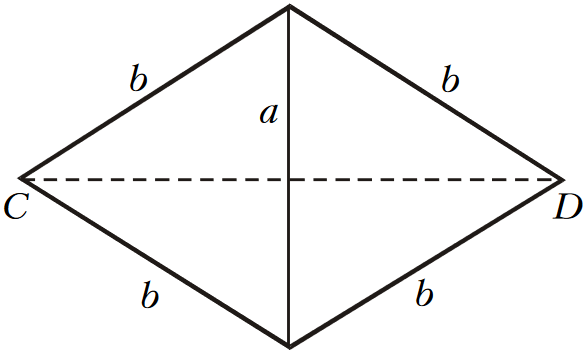
\includegraphics[width=\linewidth]{images/picture3.png} \\
\textsl{Рис. 3} \\
\end{minipage}
только тогда, когда выполнено неравенство (1),
поскольку для этого нужно, чтобы
$CD < b$
(рис.3). Убедитесь, что не существует пирамиды, три ребра
которой образуют незамкнутую ломаную. Наконец, есть еще один запрет,
так что ответ в данной задаче: 9 пирамид.\par
\textbf{Задача 7.} \textsl{Каждая из граней куба закрашивается целиком
белым или черным цветом. Раскраски двух кубов называются одинаковыми,
если эти кубы невозможно различить (при этом их разрешается
вращать в пространстве).} \par
\textsl{а) Найдите вероятность того, что при случайном раскрашивании куба все
его противоположные грани имеют различные цвета.} \par
\textsl{б) Сколько всего существует различных раскрасок куба?} \par
\textsl{в) Два художника по очереди закрашивают по одной грани куба.
Раскрасив один куб, они принимаются за следующий. Докажите,
что второй может добиться, чтобы все кубы оказались одинаково
раскрашенными.} \par
\textsl{г) Найдите вероятность того, что при случайном раскрашивании двух
кубов их раскраски оказались одинаковыми.} \par
\textbf{Решение.}  а) Поскольку вероятность того, что одна пара
противоположных граней раскрашена в противоположные цвета, равна
$\frac{1}{2}$, а а таких пар три, то ответ: $\frac{1}{3}$ \par
б) Ответ: всего имеется десять различных раскрасок. Действительно,
имеется по одной раскраске с числом белых граней, равным 0, 1, 5 или 6, и
по две раскраски, если таковых граней 2, 3 или 4. \par
в) Второй художник может действовать по следующему алгоритму:
он раскрашивает грань, противоположную той, которую перед этим
закрасил первый, причем красит ее противоположеным цветом.
\end{multicols}

\end{document}